\subsubsection{Description}
This example shows the ability to use Cellular neural networks to find edges of different objects in grey-scale picture. It uses a grey-scale picture as an input, matrix setting shown bellow(\ref{fig:EDSC}) and fixed value boundary condition to produce a binary picture with the edges.
\subsubsection{Setup}

\textbf{Input:} Grayscale picture.\\
\textbf{Boundary conditions:} Flux.\\
\textbf{Initial output:} Unimportant (all zeros)

\begin{minipage}{0.9\linewidth}
\begin{equation}
A =
\begin{bmatrix}
 0 & 0 & 0 \\
 0 & 2 & 0 \\
 0 & 0 & 0
\end{bmatrix}
B =
\begin{bmatrix}
 -1 & -1 & -1 \\
 -1 & 8 & -1 \\
 -1 & -1 & -1
\end{bmatrix}
Z = -0.5
\end{equation}
\captionof{figure}{Chosen values of A,B and Z for this experiment}
\label{fig:EDSC}
\end{minipage}


\subsubsection{Results}
Figure \ref{fig:input} show input used in this example, it is a picture with several objects of different shade of grey. The Figure \ref{fig:output} shows typical result of this experiment. This functionality is based on removing all pixels that have all only pixels with the same color around them. \\

\begin{minipage}{0.5\linewidth}
	\centering
	
\includegraphics[width=0.9\linewidth]{./Experiments/EdgeDetectionGS/fig/Input.png}
	\captionof{figure}{Input}
	\label{fig:input}
\end{minipage}
\begin{minipage}{0.5\linewidth}
	\centering
	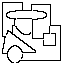
\includegraphics[width=0.9\linewidth]{./Experiments/EdgeDetectionGS/fig/Output.png}
	\captionof{figure}{Output}
	\label{fig:output}
\end{minipage}